%%%%%%%%%%%%%%%%%%%%%%%%%%%%%%%%%%%%%%%%%%%%%%%%%%%%%%%%%%%%%%%%%%%%%%%%
%    INSTITUTE OF PHYSICS PUBLISHING                                   %
%                                                                      %
%   `Preparing an article for publication in an Institute of Physics   %
%    Publishing journal using LaTeX'                                   %
%                                                                      %
%    LaTeX source code `ioplau2e.tex' used to generate `author         %
%    guidelines', the documentation explaining and demonstrating use   %
%    of the Institute of Physics Publishing LaTeX preprint files       %
%    `iopart.cls, iopart12.clo and iopart10.clo'.                      %
%                                                                      %
%    `ioplau2e.tex' itself uses LaTeX with `iopart.cls'                %
%                                                                      %
%%%%%%%%%%%%%%%%%%%%%%%%%%%%%%%%%%
%
%
% First we have a character check
%
% ! exclamation mark    " double quote
% # hash                ` opening quote (grave)
% & ampersand           ' closing quote (acute)
% $ dollar              % percent
% ( open parenthesis    ) close paren.
% - hyphen              = equals sign
% | vertical bar        ~ tilde
% @ at sign             _ underscore
% { open curly brace    } close curly
% [ open square         ] close square bracket
% + plus sign           ; semi-colon
% * asterisk            : colon
% < open angle bracket  > close angle
% , comma               . full stop
% ? question mark       / forward slash
% \ backslash           ^ circumflex
%
% ABCDEFGHIJKLMNOPQRSTUVWXYZ
% abcdefghijklmnopqrstuvwxyz
% 1234567890
%
%%%%%%%%%%%%%%%%%%%%%%%%%%%%%%%%%%%%%%%%%%%%%%%%%%%%%%%%%%%%%%%%%%%
%
\documentclass[12pt,ngerman,american]{iopart}
\newcommand{\gguide}{{\it Preparing graphics for IOP Publishing journals}}
%Uncomment next line if AMS fonts required
%\usepackage{iopams}

\usepackage[utf8]{inputenc}         % this is needed for Umlaute
\usepackage[main=american]{babel} % this is needed for Umlaute
\usepackage[T1]{fontenc}            % this is needed for correct output of umlauts in pdf
\usepackage{cite}



\usepackage[dvipsnames]{xcolor}         % Enabling colors by their 'svgnames'
\usepackage[%
  unicode=false,%
  pdftitle={A primer to numerical simulations: The perihelion motion of Mercury},%
  pdfauthor={C. K\"orber, I. Hammer, J.-L. Wynen, J. Heuer, C. M\"uller and C. Hanhart},%
  pdfkeywords={Numerical Simulations, Teaching, Perihelion Motion of Mercury, General Relativity},%
  pdfsubject={A primer with the goal to teach general concepts of numerical simulations to high school students.  The specific example is the perihelion motion of Mercury due to General Relativity.},   % subject of the document
  colorlinks=true,        % true: colored links
  linkcolor=OliveGreen,          % color of internal links (change box color with linkbordercolor)
  citecolor=magenta,        % color of links to bibliography
  filecolor=YellowGreen,      % color of file links
  urlcolor=blue           % color of external links
]{hyperref}
\usepackage[space=true]{accsupp}
% requires the latest version of package accsupp
\newcommand{\copyablespace}{\BeginAccSupp{method=hex,unicode,ActualText=00A0}\ \EndAccSupp{}}


%%%%%%%%%%%%%%%%%%%%%%%%%%%%%%%%%%%%%%%%%%%%%%%%%%%%%%%%%%%%%%%%%%%
% Custom
%%%%%%%%%%%%%%%%%%%%%%%%%%%%%%%%%%%%%%%%%%%%%%%%%%%%%%%%%%%%%%%%%%%

\usepackage{textcomp,gensymb}       % \degree

\usepackage[autostyle=true]{csquotes}            % Define quotation style
\MakeOuterQuote{"}                               % Text wrapped in "..." is recognized as a quotation

\usepackage{amssymb}                  % Math stuff
\usepackage{graphicx}                 % Import Pictures + PDFs
\usepackage{listings}                 % Code listings  See: https://en.wikibooks.org/wiki/LaTeX/Source_Code_Listings

\usepackage{subcaption} % subfigures


%%%%%%%%%%%%%%%%%%%%%%%%%%%%%%%%%%%%%%%%%%%%%%%%%%%%%%%%%%%%%%%%%%%
% Definitions
%%%%%%%%%%%%%%%%%%%%%%%%%%%%%%%%%%%%%%%%%%%%%%%%%%%%%%%%%%%%%%%%%%%
\definecolor{fzjblue}{HTML}{005B81}
\definecolor{light-gray}{gray}{0.97}
\definecolor{semilight-gray}{gray}{0.67}
\definecolor{mygreen}{rgb}{0,0.6,0}

% Custom code listings environment
\lstset{
  language=Python,
  backgroundcolor=\color{light-gray},   % choose the background color; you must add \usepackage{color} or \usepackage{xcolor}
  basicstyle=\linespread{1}\footnotesize\ttfamily,        % the size of the fonts that are used for the code
  commentstyle=\color{mygreen},
  frame=single,
  keywordstyle=\color{blue},       % keyword style
  tabsize=4,	                   % sets default tabsize to 2 spaces
  showtabs=false,
  rulecolor=\color{black},
  columns=fullflexible,
  literate={\ }{{\copyablespace}}1
}

\usepackage[prependcaption, textsize=tiny]{todonotes}

%%%%%%%%%%%%%%%%%%%%%%%%%%%%%%%%%%%%%%%%%%%%%%%%%%%%%%%%%%%%%%%%%%%
% Commands
%%%%%%%%%%%%%%%%%%%%%%%%%%%%%%%%%%%%%%%%%%%%%%%%%%%%%%%%%%%%%%%%%%%
\newcommand{\python}[0]{\texttt{Python}}
\newcommand{\vpython}[0]{\texttt{VPython}}
\newcommand{\abs}[1]{\left\vert #1 \right\vert}
\newcommand{\code}[1]{{\scriptsize\colorbox{light-gray}{\texttt{#1}}}}


%%%%%%%%%%%%%%%%%%%%%%%%%%%%%%%%%%%%%%%%%%%%%%%%%%%%%%%%%%%%%%%%%%%
% Here it starts
%%%%%%%%%%%%%%%%%%%%%%%%%%%%%%%%%%%%%%%%%%%%%%%%%%%%%%%%%%%%%%%%%%%
\begin{document}

\title[A primer to numerical simulations]{A primer to numerical simulations: The perihelion motion of Mercury}

\author{
	C.~K\"orber$^{1}$,
	I.~Hammer$^{1}$,
	J.-L.~Wynen$^{1}$,
	J.~Heuer$^{2}$,
	C.~M\"uller$^{3}$ and
	C.~Hanhart$^{1}$
}
\address{
	$^1$ \textit{Institut f\"ur Kernphysik (IKP-3) and Institute for Advanced Simulations (IAS-4), Forschungszentrum J\"ulich, D-52425 J\"ulich, Germany}\\
	$^2$ \textit{Institut f\"ur Neurowissenschaften und Medizin (INM-4), Forschungszentrum J\"ulich, D-52425 J\"ulich, Germany}\\
	$^3$ \textit{JuLab, Forschungszentrum J\"ulich, D-52425 J\"ulich, Germany}
}
\ead{c.koerber@fz-juelich.de, c.hanhart@fz-juelich.de}
\vspace{10pt}
%\begin{indented}
%\item[]February 2014
%\end{indented}

\begin{abstract}
Numerical simulations are playing an increasingly important role in modern science.
In this work it is suggested to use a numerical study of the famous perihelion motion of the planet Mercury (one of the prime observables supporting Einsteins General Relativity) as a test case to teach numerical simulations to high school students.
The paper includes details about the development of the code as well as a discussion of the visualization of the results.
In addition a method is discussed how to estimate the size of the effect a priori. Which allows to double check the results found numerically.
\end{abstract}

% Uncomment for PACS numbers
%\pacs{00.00, 20.00, 42.10}
%
% Uncomment for keywords
%\vspace{2pc}
%\noindent{\it Keywords}: XXXXXX, YYYYYYYY, ZZZZZZZZZ
%
% Uncomment for Submitted to journal title message
%\submitto{\JPA}
%
% Uncomment if a separate title page is required
%\maketitle
% 
% For two-column output uncomment the next line and choose [10pt] rather than [12pt] in the \documentclass declaration
%\ioptwocol
%

%%%%%%%%%%%%%%%%%%%%%%%%%%%%%%%%%%%%%%%%%%%%%%%%%%%%%%%%%%%%%%%%%%%
\section{Introduction}\label{sec:intro}
%%%%%%%%%%%%%%%%%%%%%%%%%%%%%%%%%%%%%%%%%%%%%%%%%%%%%%%%%%%%%%%%%%%

Numerical simulations play a key role in modern physics for they allow one to tackle theoretical problems not accessible otherwise. This might be the case because there are too many particles participating in the system (as in simulations for weather predictions) or the interactions are too complicated to allow for a systematic, perturbative approach (as in theoretical descriptions of nuclear particles at the fundamental level).
This paper introduces a project that allows one to demonstrate the power of numerical simulations.
On the example of the perihelion motion of the planet Mercury the students are supposed to learn about
\begin{itemize}
\item the importance of differential equations in theoretical physics;
\item the numerical implementation of Newtonian dynamics;
\item systematic tests and optimization of computer codes;
\item effective tools to estimate the result a priori as an important cross check;
\item the visualization of numerical results using \vpython{}.
\end{itemize}
We are convinced that in order to excite students for numerical simulations it is compulsory to demonstrate their power on an example that catches their interest.
This purpose is served perfectly by the case chosen here, since Einsteins equations of General Relativity are fascinating to a very broad public.
Their detailed study needs a deep knowledge of Differential Geometry. For the study outlined here, however, very little math is necessary, such that high school students familiar to derivatives benefit from it.
This was already demonstrated in the "Sch\"ulerakademie Teilchenphysik", where this course was tested successfully on two groups consisting in total of 24 German high school students from 10$^{\rm th}$ to 13$^{\rm th}$ grade in 2015 and 2017.

The course as well as this paper is structured as follows: after an introduction to Newtonian dynamics and the concept of differential equations, their
discretization is discussed based on Newton's law of gravitation and possible extensions thereof.
Afterwards the visualization of the resulting trajectories using \vpython{} is introduced and applied to the problem at hand. In addition,
 tools are developed to extract the relevant quantity from the result of the simulation.
Finally, the principle of dimensional analysis is presented as a tool not only to estimate some effect but also to cross check whether the results of the simulation are sensible.




%%%%%%%%%%%%%%%%%%%%%%%%%%%%%%%%%%%%%%%%%%%%%%%%%%%%%%%%%%%%%%%%%%%
\section{Trajectories, velocities, accelerations and Newton's second law}\label{sec:tva}
%%%%%%%%%%%%%%%%%%%%%%%%%%%%%%%%%%%%%%%%%%%%%%%%%%%%%%%%%%%%%%%%%%%

A physical system is said to be understood if the assumed forces acting on it lead to the observed trajectories.
In other words, we need to show that we can calculate the location in space of the object of interest at any point in time, once the initial conditions are fixed properly.
If we can neglect the finite size of this object (and in particular its orientation in space), the location is parametrized by a single three vector $\vec r(t)$.
Additionally, we need to be able to calculate the objects velocity $\vec v(t)$ and acceleration $a(t)$ in order to describe and control its dynamics; this will become clear below. The velocity describes a change of location over time which, for some infinitesimally small $\Delta t$, can be written as
\begin{equation}\label{eq:x_update}
\vec r(t+\Delta t) = \vec r(t) + \vec v(t) \Delta t + \ldots \ . \label{eq:vdef}
\end{equation}
Similarly, the acceleration describes a change in velocity, i.e.
\begin{eqnarray}\label{eq:v_update}
\vec v(t+\Delta t) = \vec v(t) + \vec a(t) \Delta t + \ldots\ . \label{eq:adef}
\end{eqnarray}
The dots in these expressions indicate additional terms that may be expressed in terms of higher powers in $\Delta t$. While they are needed in general, for sufficiently small $\Delta t$ they can be safely neglected.
Thus we may define the time derivative via
\begin{equation}
\vec v(t) = \lim_{\Delta t\to 0} \frac{\Delta \vec r(t)}{\Delta t} =: \frac{d\vec r(t)}{d t}  = \dot{\vec  r}(t) \ ,
\end{equation}
where $\Delta \vec r(t)=\vec r(t+\Delta t)-\vec r(t)$ and we introduced a common short hand notation for time derivatives in the last expression.
Analogously we get
\begin{eqnarray}
\vec a(t) &=& \lim_{\Delta t\to 0} \frac{\Delta \vec v(t)}{\Delta t} =: \frac{d\vec v(t)}{dt}  = \dot{\vec v}(t) \ , \\
 &=& \frac{d^2\vec r(t)}{dt^2}  = \ddot{\vec r}(t) \ ,
\end{eqnarray}
where we introduced the second derivative in the second line.

It was Newton who observed that if a body is at rest, it will remain at rest, and if it is in motion it will remain in motion at a constant velocity in a straight line, unless it is acted upon by some force --- this is known as Newton's first law.
Formulated differently: a force $\vec F$ expresses itself by changing the motion of some object.
This is quantified in Newton's second law
\begin{equation}
\vec F(\vec r, t) = \frac{d}{dt}(m \vec v) \ .
\end{equation}
If the mass does not change~\footnote{%
	A well known example where $m$ does change with time is a rocket, whose mass decreases as fuel is burned.
} with time, this reduces to the well known
\begin{equation}
\vec F(\vec r) = m \vec a(t) = m\dot{\vec v}(t) = m\ddot{\vec{r}}(t) \ . \label{eq:newton2}
\end{equation}
Note that in general the force could depend also on the time or the velocity.
Here, we restrict ourselves to the case relevant for our example, where the force depends on the location only.
Therefore, as soon as the force $\vec F(\vec r)$ is known for all $\vec r$ one can in principle calculate the trajectory, e.g., solving Eq.~(\ref{eq:newton2}) for $\vec r(t)$.
Sometimes this requires some advanced knowledge of mathematics and sometimes no closed form solution exists.
However, alternatively one can calculate the whole trajectory of some test body that experiences this force by a successive application of the rules given in Eqs.~(\ref{eq:vdef}) and (\ref{eq:adef}):
\begin{enumerate}
\item For a given time $t$, where $\vec r(t)$ and $\vec v(t)$ are known, use the force to calculate $\vec a(t) = \vec F(\vec r(t)) / m$, see Eq.~(\ref{eq:newton2}).
\item Use Eq.~(\ref{eq:vdef}) to calculate $\vec r(t+\Delta t)$.
\item Use Eq.~(\ref{eq:adef}) to calculate $\vec v(t+\Delta t)$.
\item Go back to (i) with $t\to t+\Delta t$.
\end{enumerate}
Clearly to initiate the procedure at some time $t_0$ both $\vec r(t_0)$ as well as $\vec v(t_0)$ must be known --- the  trajectories depend on these initial conditions~\footnote{%
	In general, a differential equation of $n^{\rm th}$ degree (where the highest derivative is order $n$) needs $n$ initial conditions specified.
	For $n=2$ those are often chosen as location and velocity at some starting time, but one may as well pick two locations at different times.%
}.

This procedure can only work if $\Delta t$ is sufficiently small.
What this means depends on the process one studies.
One way to estimate whether $\Delta t$ is small enough, is to verify whether the relation
\begin{equation}
|\vec v(t)| \gg \frac12|\vec a(t)|\Delta t = \frac{1}{2m} |\vec F(\vec r(t)) |\Delta t\
\label{eq:check}
\end{equation}
holds. This follows from Eq.~(\ref{eq:vdef}) where the first term that we neglected reads $(1/2)a(t){(\Delta t)}^2$.
Eq.~({\ref{eq:check}}) also shows that small (large) time steps are necessary (sufficient), if the force is strong (weak), since the time steps need to be small enough that all changes induced by the force get resolved.
Clearly, a relation as Eq.~({\ref{eq:check}}) can only provide guidance and can not replace a careful numerical check of the solutions: A valid result has to be insensitive the concrete value chosen for $\Delta t$ --- in particular replacing $\Delta t$ by $\Delta t/2$ should not change the result significantly.



%%%%%%%%%%%%%%%%%%%%%%%%%%%%%%%%%%%%%%%%%%%%%%%%%%%%%%%%%%%%%%%%%%%
\section{Example: General Relativity and the perihelion motion of Mercury}\label{sec:gr}
%%%%%%%%%%%%%%%%%%%%%%%%%%%%%%%%%%%%%%%%%%%%%%%%%%%%%%%%%%%%%%%%%%%
For this concrete example the starting point for the force is Newton's law of gravitation
\begin{equation}
\vec F_N(\vec r) = - \frac{G_N m M_\odot}{r^2} \frac{\vec r}{r}\ ,
\end{equation}
where $G_N=6.67\times 10^{-11}$ m$^3$kg$^{-1}$s$^{-2}$ is the Newtonian constant of gravitation, $m$ is the mass of Mercury and $M_\odot=1.99\times 10^{30}$ kg is the mass of the Sun.
In addition $r=|\vec r(t)|$ denotes the distance between Sun and Mercury when we assume that the Sun is infinitely heavier than Mercury and located at the center of the coordinate system.
Although this is not exact, it is a pretty good approximation because $m/M_\odot\sim 10^{-8}$.
For later convenience we introduce the Schwarzschild radius of the Sun
\begin{equation}
r_S=\frac{2G_N  M_\odot}{c^2} = 2.95 \ \mbox{km} \ , \label{rsdef}
\end{equation}
where $c=3.00\times 10^8$ m/s denotes the speed of light.
Note that $r_S$ is the characteristic length scale of the gravitational field of the Sun for --- up to the prefactor --- one can not form another quantity with dimensions of a length from $G_N$, $M_\odot$ and $c$.
The Schwarzschild radius is also an important quantity to characterize black holes; this is however not relevant for the discussion at hand.
With this, Newton's second law reads
\begin{equation}
\ddot{\vec r}      = - \frac{c^2}{2}\left(\frac{r_S}{r^2}\right)\frac{\vec r}{r} \, . \label{eq:newton}
\end{equation}
An attractive force that vanishes at large distances leads in general, depending on the initial conditions, either to bounded or to open orbits.
In the latter case the planet simply disappears from the Sun, since a given force can capture only bodies with small enough momenta.
The students may study those scenarios within their simulations by varying the start velocity while keeping the start location fixed.

The bounded orbits that emerge from a potential that scales as $1/r$ (which corresponds to a force that scales as $1/r^2$) are elliptic and fixed in space.
In particular the point of closest approach of the planet to the Sun, the perihelion, does not move.
However, when a potential that vanishes for $r\to \infty$ deviates from $1/r$, the perihelion does move.
This makes the behavior of the perihelion a very sensitive probe of the gravitational potential.

The observed perihelion motion of Mercury is nowadays determined as
\[(574.10\pm 0.65)'' \ \mbox{per 100 earth years \cite{RevModPhys.19.361}}\]
where the symbol $''$ denotes "arc seconds": 1$''={(1/3600)}^o$. The bulk of this number
can be understood by the presence of other planets within the Newtonian theory, since
their gravitational force also acts on Mercury. However, a
residual motion of
\begin{equation}
\delta \Theta_M = (43)'' \ \mbox{in 100 earth years} \label{delT}
\end{equation}
remained unexplained, until Einstein quantified the predictions of General Relativity to this particular observable~\cite{Einstein}.

To allow for a movement of the perihelion we need to modify the force that led to Eq.~(\ref{eq:newton}).
This modification should be such that it depends on $r$ and it vanishes for $r\to \infty$.
Based on the discussion presented above we may multiply the right hand side of~(\ref{eq:newton}) with a factor
$(1+\alpha(r_S/r))$, where $\alpha$ denotes some dimensionless parameter.
This seems like a natural way to parametrize the additional potential because it adds the smallest possible deviation from an $1/r$ potential expressed relative to the characteristic length $r_S$.
However, besides $r_S$, which characterizes the gravitational potential of the Sun, there is also a characteristic parameter for the dynamics of Mercury:
\begin{equation}
r_a^2 := \frac{\vec L\,^2}{m^2c^2}= \frac{{(\vec r\times \dot{\vec r} \, )}^2}{c^2} \ , \label{a2def}
\end{equation}
where $\vec L$ denotes the angular momentum, which is a constant of motion for central potentials.
It is easily verified that $r_a^2$ carries dimensions of length squared.
We therefore have to add one more term to the potential; in analogy to the one discussed above, we use $\beta (r_a^2/r^2)$.
Combining everything, we use the following ansatz for the modified equation of motion:
\begin{equation}
\ddot{\vec r} = - \frac{c^2}{2}\frac{r_S}{r^2}\left(1+\alpha\frac{r_S}{r}+\beta\frac{r_a^2}{r^2}\right) \, \frac{\vec{r}}{r} \ .
\label{eq:newton_art}
\end{equation}
For the system at hand, $r_a^2$ may be estimated from the parameters of Mercury at its perihelion: The corresponding velocity is
 $\dot{\vec r}(t=0)=\abs{\vec v_M(0)} = 59.0$~km/s (here we already indicate that we will start the simulation at the perihelion) and the closest distance between Sun and Mercury is
$ r_{MS}=\abs{\vec r_{MS}(0)} = 46.0 \cdot 10^6$km~\cite{MercuryFactSheet}. Note that at the perihelion $\vec r$ and $\dot{\vec r}$ are perpendicular to each other.
We thus find that $(r_a^2/ r_{MS}^2) \sim 4\cdot10^{-8}$. Furthermore $(r_S/r_{MS})\sim6\cdot 10^{-8}$.
Therefore (for a more detailed discussion about the underlying logic we refer to Sec.~\ref{sec:analysis}) one may expect from both correction terms an effect of similar size. Furthermore, any term of higher order in either $a$ or $r_S$
should be suppressed by additional seven orders of magnitude and thus can be neglected safely.
The parameters $\alpha$ and $\beta$ can be extracted from a fit to data --- this will be done below.
However, since we have only a single number to study, the perihelion shift (see Eq.~(\ref{delT})),
we can only fix either $\alpha$ or $\beta$ (or a linear combination thereof).
The parameters can also be calculated from the underlying theory one uses. The actual values depend on the specific theory;
General relativity gives~\cite{Einstein}
\begin{equation}
	\alpha = 0 \, , \quad \beta = 3 \, . \label{eq:art-prediction}
\end{equation}
Thus we may also use the simulation explained below to calculate the perihelion motion of Mercury from the input
values given in Eq.~(\ref{eq:art-prediction}).


% For comparison: the typical distance of the Venus, the neighbor of Mercury, to the sun is $(r_S/r_{VS}) \sim 5 \cdot 10^{-8}$.
% Therefore the expected ratio of residual motion, favoring in the orbit period $T$, would result in
% \begin{equation}
% 	\delta \Theta_V \approx \frac{1}{T_V} \delta \Theta_M T_M \frac{r_{MS}}{r_{VS}} \approx 9'' \, ,
% \end{equation}
% where $T_V$ ($T_M$) denotes the length of a venus (Mercury) year. This precisely describes the experimental value of $9''$.



%%%%%%%%%%%%%%%%%%%%%%%%%%%%%%%%%%%%%%%%%%%%%%%%%%%%%%%%%%%%%%%%%%%
\section{Numerical Implementation}\label{sec:Numerical Implementation}
%%%%%%%%%%%%%%%%%%%%%%%%%%%%%%%%%%%%%%%%%%%%%%%%%%%%%%%%%%%%%%%%%%%

%------------------------------------------
\subsection{Describing the Motion with Python}
%------------------------------------------

In this section we present the numerical implementation as well as the visualization of planetary trajectories and in
particular the perihelion motion of Mercury.
We choose \python{}~\cite{Python} as programming language because \python{} is easy to learn, intuitive to understand and an open source language.
No prior knowledge of \python{} or any other programming language is required, as we explain all necessary steps to create the simulation.
We provide online instructions for setting up \python{} and \vpython{} on different operating systems \cite{scripts}.
In \ref{sec:code}, we also provide a working example as well as possible extensions and template files online.

To start the simulation one needs the "initial" distance and velocity [Eq.~(\ref{eq:x_update}) and Eq.~(\ref{eq:v_update})].
As described above, here one can simplify the problem by placing one object (the "infinitely" heavy Sun) in the center of the coordinate system and keep it fixed.

Since the trajectories do not depend on where on the orbit of Mercury the simulation is started, we
use the values at the perihelion with $\abs{\vec r_{MS}(0)} = 46 \cdot 10^6\,\mathrm{km}$ and $\abs{\vec v_M(0)} = 59\,\mathrm{km/s}$\cite{MercuryFactSheet} as initial (for $t=0$) parameters.
The computer does not understand physical units, hence one has to express each variable in an appropriate unit.
Both for the numerical treatment and the intuitive understanding, it is useful to select parameters in a "natural range", e.g.,
by expressing distances in $R_0 = 10^{10}\,\mathrm{m}$ and time intervals in days, $T_0 = 1\,\mathrm{d}$, where d refers to earth days. One Mercury year is given by $T_M=88.0\,T_0$.
With this choice, the initial distance of Mercury to the Sun, the size of the initial velocity of Mercury and the acceleration prefactor (see Eq.~(\ref{eq:newton_art})) become
\begin{eqnarray}
r_{MS}(0)   &=& 4.60 R_0 \, , \quad
v_{M}(0)    = 0.510 \frac{R_0}{T_0} \, ,  \\
a_{MS}(r_{MS}) &=& \frac{c^2}{2}\frac{r_S}{r^2} = 0.990 \frac{R_0}{T_0^2} \frac{1}{{\left(r_{MS}/R_0\right)}^2}\, .
\end{eqnarray}

%
\begin{figure}[htb]
	\centering
	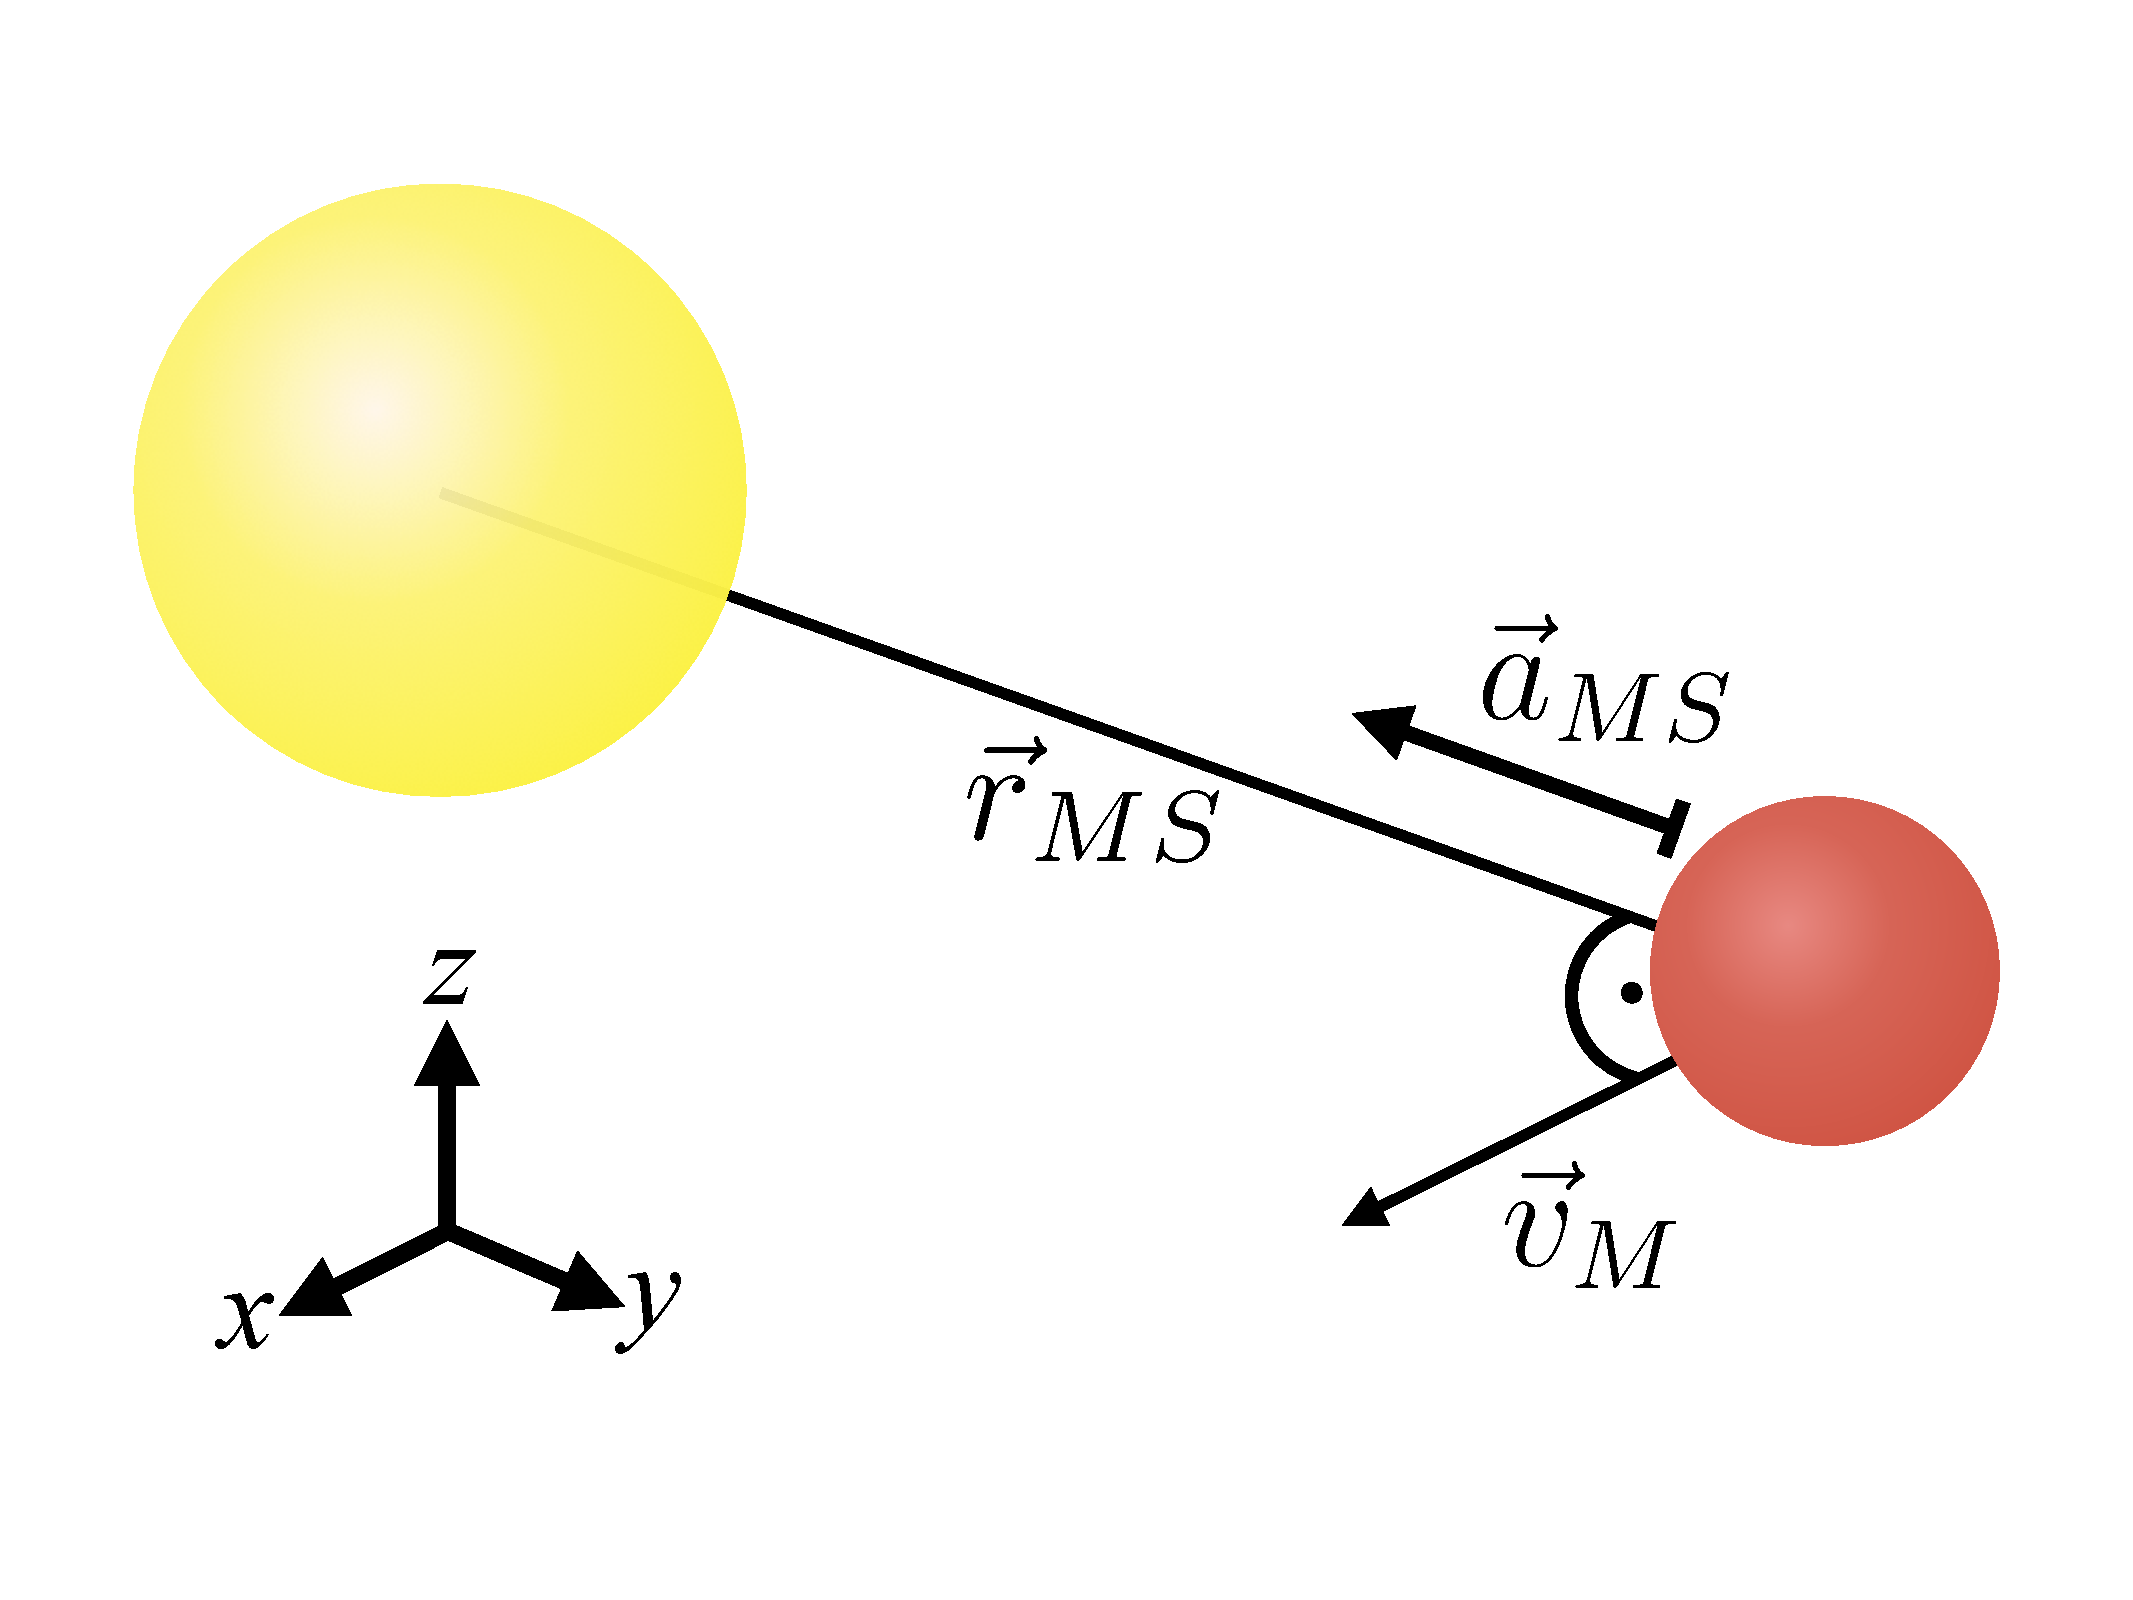
\includegraphics[width=.5\textwidth]{figs/sun_merc.pdf}
	\caption{\label{fig:sun_merc}%
		Sun-Mercury system with relevant vectors.
		Mercury is at its perihelion, therefore its velocity is perpendicular to its direct connection vector with the sun.%
	}
\end{figure}
%

In \python{}, this reads
\begin{lstlisting}
# Definition of parameters
rM0 = 4.60    # initial radius of Mercury orbit, in units of R0
vM0 = 5.10e-1 # initial orbital speed of Mercury, in units of R0/T0
c_a = 9.90e-1 # base acceleration of Mercury, in units of R0**3/T0**2
TM  = 8.80e+1 # Orbit period of Mercury
rS  = 2.95e-7 # Schwarzschild radius of Sun,in units of R0
ra2 = 8.19e-7 # specific angular momentum, in units of R0**2
\end{lstlisting}
where $\texttt{c\_a} =a_{MS} r_{MS}^2$, the acceleration without the radius factor.
The last two quantities refer to the Schwarzschild radius of the Sun and the parameter $r_a^2$ defined in Eqs. (\ref{rsdef}) and (\ref{a2def}), respectively.

So far we only fixed the length of the vectors. Next, we set up the initial directions, which will describe the motion in space.
We will build on the existing \python{} module \vpython{}, which provides an implementation for treating vectors as well as their visualization.
The first object of interest is a \texttt{vector}, which takes three-dimensional coordinates as its input.
With our choice of initial conditions (we picked the initial vectors in the perihelion), the velocity of Mercury is perpendicular to the vector which connects Mercury and Sun (see figure~\ref{fig:sun_merc}):
\begin{lstlisting}
# Import the class vector from vpython
from vpython import vector
# Initialize distance and velocity vectors
vec_rM0 = vector(0, rM0, 0)
vec_vM0 = vector(vM0, 0, 0)
\end{lstlisting}
We use the estimate of Eq.~(\ref{eq:check}) as a guidance to fix the time step $\Delta t$ as
\begin{lstlisting}
# Definition of the time step
dt = 2 * vM0 / c_a / 20
\end{lstlisting}
Here the factor $1/20$ makes sure that $\Delta t$ is indeed consistent with Eq.~(\ref{eq:check}).
Now we are in the position to calculate location and velocity of the planet at $t_0+\Delta t$ using the following expressions\footnote{%
	Note, that there are different notions for numerically integrating differential equations with different accuracies.
	Thus, the ordering and exact expressions for updating $a_{MS}$, $v_M$ and $r_{MS}$ are not unique. However, all correct prescriptions lead to the same result for sufficiently small $\Delta t$.
	For this particular problem, the definitions we show are in good balance between being numerically stable and inexpensive to compute.
}%
\begin{lstlisting}
# Compute the strength of the acceleration
temp = 1 + alpha * rS / vec_rM_old.mag + beta * ra2 / vec_rM_old.mag**2
aMS  = c_a * temp / vec_rM_old.mag**2
# Multiply by the direction
vec_aMS = - aMS * ( vec_rM_old / vec_rM_old.mag )
# Update velocity vector
vec_vM_new = vec_vM_old + vec_aMS * dt
# Update position vector
vec_rM_new = vec_rM_old + vec_vM_new * dt
\end{lstlisting}
Note basic vector operations are already implemented in the predefined \texttt{vector} class.
The difference and sum of two vectors, or the scalar vector multiplication return vectors themselves.
Also the magnitude of a vector --- \code{vector.mag} --- is an attribute of the vector and can be easily extracted.

It is handy to use \texttt{Python}s functions to structure the program and hold repeating code ("DRY" --- Don't Repeat Yourself):
\begin{lstlisting}
# Define the coordinate and velocity update function
def evolve_mercury(vec_rM_old, vec_vM_old, alpha, beta):
    # Compute the strength of the acceleration
    temp = 1 + alpha * rS / vec_rM_old.mag + beta * ra2 / vec_rM_old.mag**2
    aMS  = c_a * temp / vec_rM_old.mag**2
    # Multiply by the direction
    vec_aMS = - aMS * ( vec_rM_old / vec_rM_old.mag )
    # Update velocity vector
    vec_vM_new = vec_vM_old + vec_aMS * dt
    # Update position vector
    vec_rM_new = vec_rM_old + vec_vM_new * dt
    return vec_rM_new, vec_vM_new

# Call the function
vec_rM_new, vec_vM_new = evolve_Mercury(vec_rM_old, vec_vM_old, 0.0, 0.0)
\end{lstlisting}
\python{}s syntax enforces a clean programming style: it is necessary that the body of the function is indented (by an arbitrary but consistent amount of \texttt{space}s\footnote{While \python{} allows using \texttt{tab}s as well, this can cause programming errors, because their displayed width depends on the text editor.}) relative to the definition statement of the function.
Furthermore, \python{} is an Interpreter language.
Each line of the code is executed when the Interpreter passes it.
For this reason, if we define the parameters before the function, they can be used inside of the function.
Variables defined within the function (e.g. \code{aMS}, \code{vec\_aMS}, $\dots$) are local and do not exist beyond the scope of the function; they can not be used after the \texttt{return} statement.

Finally, we can describe the evolution by a \texttt{while}-loop
\begin{lstlisting}
t     = 0.0
alpha = 0.0
beta  = 0.0
# Set position and velocity to their starting points
vec_rM = vec_rM0
vec_vM = vec_vM0
# Execute the loop as long as t < 2*TM
while t < 2*TM:
    # Update position and velocity
    vec_rM, vec_vM = evolve_mercury(vec_rM, vec_vM, alpha, beta)
    # Advance time by one step
    t = t + dt
\end{lstlisting}
where for the start we set the parameters $\alpha=0 = \beta$ in order to first study the properties of the pure
$1/r^2$ force.
Note the required indent of the loop structure similar to the indent of a function.
In each iteration of the \texttt{while}-loop, the previous distance and velocity are used to compute the new values,
directly overwriting the previous values.
The total runtime \texttt{2*TM} is the amount of "virtual" days the simulations should run.
To describe at least one full orbital period, this time needs to be larger than $T_M$.
With the previous choice for \texttt{dt}, this corresponds to roughly $N_T \approx 2 \cdot 10^3$ evolution steps.
Note that the exact time it takes for Mercury to complete a full revolution depends on the initial coordinates and velocities, the accuracy of the computation
(controlled by the value of $\Delta t$) as well as the computing power employed.
One should encourage the students to analyze this in the beginning.

%------------------------------------------
\subsection{Visualizing the Motion with VPython}
%------------------------------------------
To start the visualization one has to \texttt{import} further objects from the \texttt{VPython} module.
We change the import statement from before to
\begin{lstlisting}
from vpython import vector, sphere, color, curve, rate
\end{lstlisting}
The class sphere will represent Mercury and the Sun in the simulation
\begin{lstlisting}
# Define the initial coordinates; M = Mercury, S = Sun
M = sphere(pos=vec_rM0,       radius=0.5,  color=color.red   )
S = sphere(pos=vector(0,0,0), radius=1.5,  color=color.yellow)
# And the initial velocities
M.velocity = vec_vM0
S.velocity = vector(0,0,0)
# Add a visible trajectory to Mercury
M.trajectory = curve(color=color.white)
\end{lstlisting}
We place the Sun in the origin of our coordinate system and choose non-realistic radii for visualization purposes.
Last but not least, one should the vectors related to the visualization directly instead of extra vectors as was done before. Thus
the \texttt{while}-loop becomes
\begin{lstlisting}
t     = 0.0
alpha = 0.0
beta  = 0.0
# Execute the loop as long as t < 2*TM
while t < 2*TM:
    # Set the frame rate (you can choose a higher rate to accelerate the program)
    rate(100)
    # Update the drawn trajectory with the current position
    M.trajectory.append(pos=M.pos)
    # Update velocity and position
    M.pos, M.velocity = evolve_mercury(M.pos , M.velocity , alpha, beta)
    # Advance time by one step
    t = t + dt
\end{lstlisting}

If the starting values are chosen as advised in the previous section, the students should end up with a trajectory as depicted in figure~\ref{fig:MercuryOrbit-a0-small}.
At this point one might ask students to vary $\Delta t$ and observe the effect of this on the orbit [see also figure~\ref{fig:MercuryOrbit-a0-small-dt-large}].
To get the perihelion motion, the additional force term described in Eq.~(\ref{eq:newton_art}) has to be "turned on", e.g., by choosing  $\alpha\neq0$
[figure~\ref{fig:MercuryOrbit-a6-small}].
This is a good opportunity to let the students play with the size of $\alpha$ and get a feeling for its impact on the trajectories. In particular
they should discover that values of $\alpha$ of the order of $10^6$ are necessary to get a visible effect.
For a nicely visible perihelion motion it is advisable to not use the correct Mercury values but a more excentric trajectory by choosing, e.g., $r_{MS}(0)=6R_0$ [figure~\ref{fig:MercuryOrbit-a6-big}].
\begin{figure}[htb]
	\centering
	\begin{subfigure}[c]{0.22\textwidth}
		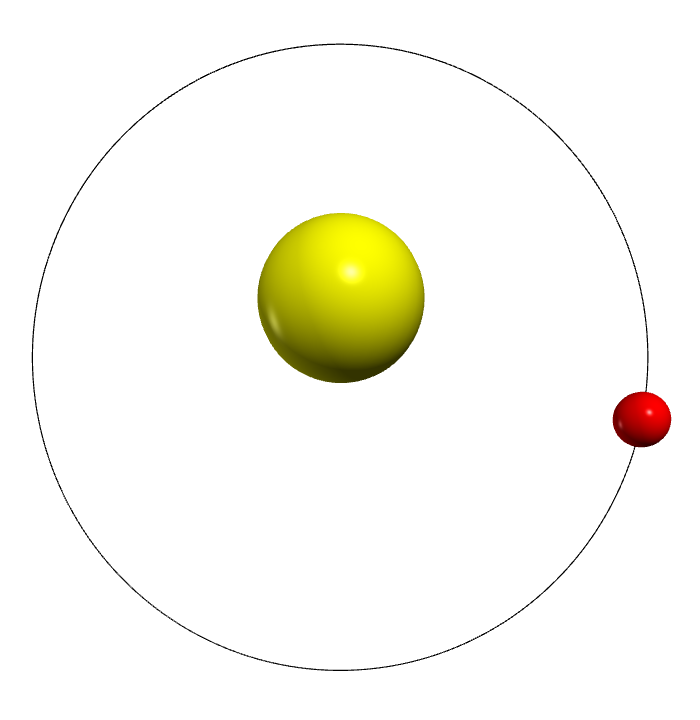
\includegraphics[width=\textwidth]{figs/a0T5dt20.png}
		\caption{\label{fig:MercuryOrbit-a0-small}}
	\end{subfigure}
	~
	\begin{subfigure}[c]{0.22\textwidth}
		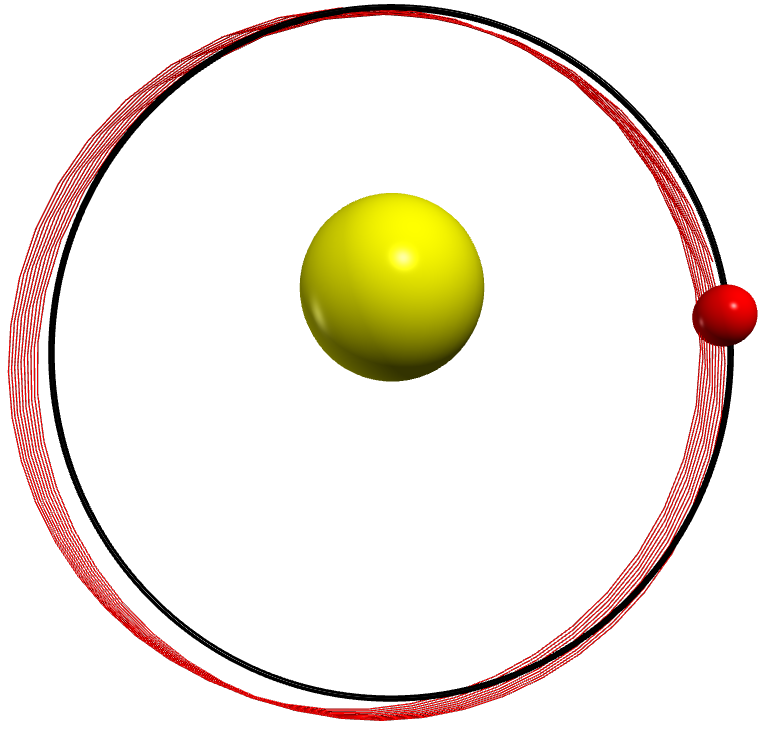
\includegraphics[width=\textwidth]{figs/num-err.png}
		\caption{\label{fig:MercuryOrbit-a0-small-dt-large}}
	\end{subfigure}
	~
	\begin{subfigure}[c]{0.22\textwidth}
		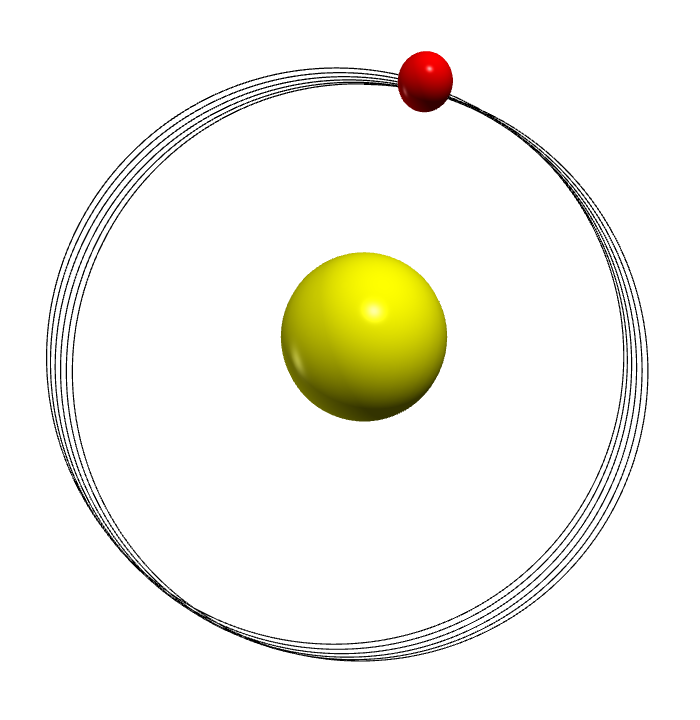
\includegraphics[width=\textwidth]{figs/a6T5dt20.png}
		\caption{\label{fig:MercuryOrbit-a6-small}}
	\end{subfigure}
	~
	\begin{subfigure}[c]{0.22\textwidth}
		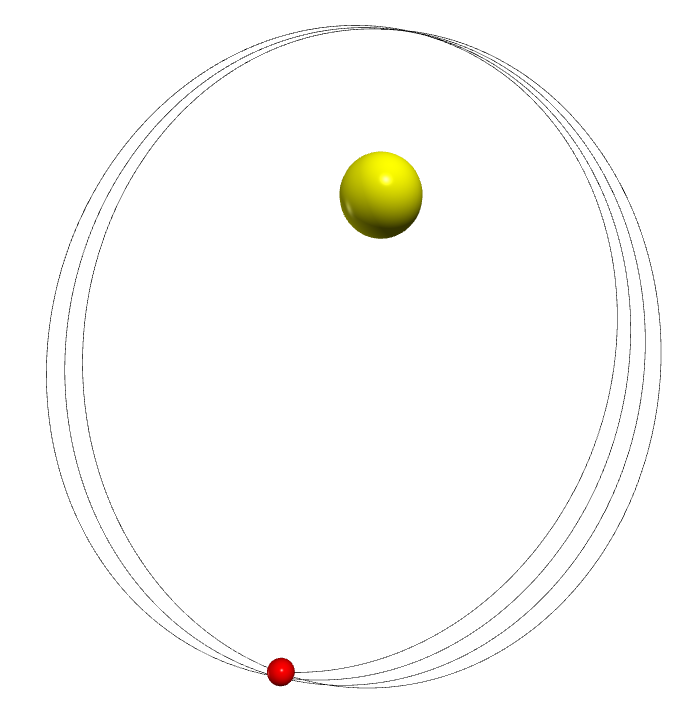
\includegraphics[width=\textwidth]{figs/a6T10dt20.png}
		\caption{\label{fig:MercuryOrbit-a6-big}}
	\end{subfigure}
	\captionsetup{singlelinecheck=off}
	\caption[]{\label{fig:MercuryOrbit}
		Different Mercury orbits for $\beta=0$ and
		\begin{itemize}
		\item[(a)] $\alpha=0$ and $\Delta t = \Delta t_0  / 20$;
		\item[(b)] $\alpha=0$ and $\Delta t = \Delta t_0  \times 2$, where the black line represents the orbit of (a) and the red line is the orbit for the larger time steps;
		\item[(c)] $\alpha=10^{6}$ and $\Delta t = \Delta t_0 / 20$;
		\item[(d)] $\alpha=10^{6}$ and $\Delta t = \Delta t_0 / 20$ but $r_{MS}(0) = 6 R_0$.
		\end{itemize}
		Here, the time steps are defined by $\Delta t_0 \equiv 2 v_{M}(0) /a_M(0)$ and the images are screenshots of the simulation (with modified colors).
		Note that for different starting values of $r_{MS}(0)$, also the numbers of days for a "Mercury year" changes.
	}
\end{figure}

%------------------------------------------
\subsection{Extracting the Perihelion Motion}
%------------------------------------------

%\textit{What exactly do we want the students / advise the teachers to do? I think a nice approach would be to let the students implement the code to extract the perihelion motion and make a list of some values of alpha and the corresponding angles. Then discuss, that $\alpha=1$ is the natural size for $\alpha$ and that to extract the value of angle they need to exploit the linear dependence. Finally they can think on whether the value they get is reasonable and the teacher can explain the rest of section? What do you think?}\\
Both $\alpha$ and $\beta$ have similar effects on the perihelion motion.
We recommend setting one of them to zero and varying the other when analyzing the perihelion motion in dependence on the parameters.
In order to calculate the size of the perihelion motion for a modified gravitational force, the students need to
\begin{itemize}
\item extract multiple positions of the perihelion $\vec r_{MS} ( t_\mathrm{ph}^{(n)} )$ for a fixed value of $\alpha$ and $\beta$. The  simulation time needs to cover several revolutions.
\item calculate the angle between the perihelions for each pair of successive turns and compute the average angle $\delta \Theta (\alpha)$ over all individually computed angles.
\item repeat the steps given above for different values of $\alpha$ (or $\beta$). The students should find a linear dependence of $\delta \Theta$ on $\alpha$ or $\beta$.
\item interpolate $\delta \Theta (\alpha, \beta)$ to small values of $\alpha$ (or $\beta$) --- including  $\delta \Theta(0,0)=0$.
\end{itemize}

There are several ways to find the position of the perihelion.
The easiest one is to look for the point of minimal distance to the sun --- the definition of the perihelion.
This can be done within the $while$-loop.
To identify a minimal distance to the sun, one has to know the last two positions \code{vec\_rM\_past} and \code{vec\_rM\_before\_last} in addition to the current position.
If the length of the \texttt{last} vector is smaller than that of the \texttt{before\_last} vector and smaller than the current vector, one has passed the perihelion and its position is given by \code{vec\_r\_last}.
It is useful to save the position of the perihelion in a list \code{list\_perih} for a certain number of turns (here e.g.\ \code{max\_turns = 10}).
The implementation can be realized as follows\footnote{%
	Note that one stores \code{vec\_r\_last} by making a copy of \code{M.pos}: \code{vec\_r\_last = vector(M.pos)}.
	This is essential because otherwise, if one changes \code{M.pos}, one would automatically change \code{vec\_r\_last} as well.
}
\begin{lstlisting}
# Set up vectors
vec_rM_last = vec_rM0
turns      = 0
max_turns  = 10
list_perih = list()
# Find perihelion for each turn and print it out
while turns < max_turns:
    vec_rM_before_last = vec_rM_last
    # Store position of Mercury in a new vector (since we will change M.pos)
    vec_rM_last = vector(M.pos)
    #<...update Mercury position...>
    # Check if at perihelion
    if (vec_rM_last.mag < M.pos.mag) and (vec_rM_last.mag < vec_rM_before_last.mag):
        list_perih.append(vec_rM_last)
        turns = turns + 1
\end{lstlisting}
The angle between two vectors can be computed using
 \begin{equation}
 	\sphericalangle(\vec{v}_{1},\vec{v}_2) = \mathrm{arccos} \left( \frac{\vec{v}_{1} \cdot \vec{v}_2}{|\vec{v}_{1}|\:|\vec{v}_2|} \right)
	\, .
 \end{equation}
This is readily implemented in \texttt{VPython} via
\begin{lstlisting}
# Import functions to compute angle
from vpython import acos, pi, dot
# Define function for angle extraction
def angle_between(v1, v2):
    return acos( dot(v1, v2) / (v1.mag * v2.mag) ) * 180. / pi
\end{lstlisting}
where the factor $180/\pi$ in the last line converts the unit of the angle from radians into degrees.
To account for the statistical errors (e.g.\ numerical rounding errors) one can average over a few turns.
Depending on the programming proficiency of the students and time constraints, this can be done either by hand or, e.g., by implementing the following code
\begin{lstlisting}
sum_angle=0.
for n in range(1, max_turns):
    # Calculate angle
    sum_angle = sum_angle + angle_between(list_perih[n-1], list_perih[n])
# Display the average
print(sum_angle/(max_turns-1))
\end{lstlisting}
Note that the perihelion motion is computed from the locations stored in \code{list\_perih} and not based on the initial position.
This is important because depending on the initial conditions and numerical uncertainties, the simulation does not necessarily start in the perihelion.

As explained above [and further discussed in chapter~\ref{sec:analysis}] the natural value for $\alpha$ would be of the order of $1$.
However, if the students use this value for $\alpha$, they will find that the change in the trajectories is close to invisible and the numerical uncertainty is much larger than the result.
It is therefore more advisable to use the fact that there is a linear dependence between $\alpha$ and $\delta \Theta$ to estimate the size of the perihelion motion\footnote{%
	Of course for very large values of $\alpha$ this linear relation will eventually break down.
	We therefore advise to choose $\alpha<7\cdot 10^6$ at which point the perihelion motion exceeds $\delta \Theta=90^{\degree}$.
}.
The students can convince themselves of this fact by plotting the angles $\delta \Theta$ they have extracted from their simulation over $\alpha$.
This can be done either by hand, \python{} (e.g., with \texttt{matplotlib}~\cite{Matplotlib}), or using another program like, e.g., Excel.
For instance figure~\ref{fig:AlphaAngle} demonstrates such a plot.

\begin{figure}[htb]
	\centering
	\begin{subfigure}[c]{0.49\textwidth}
		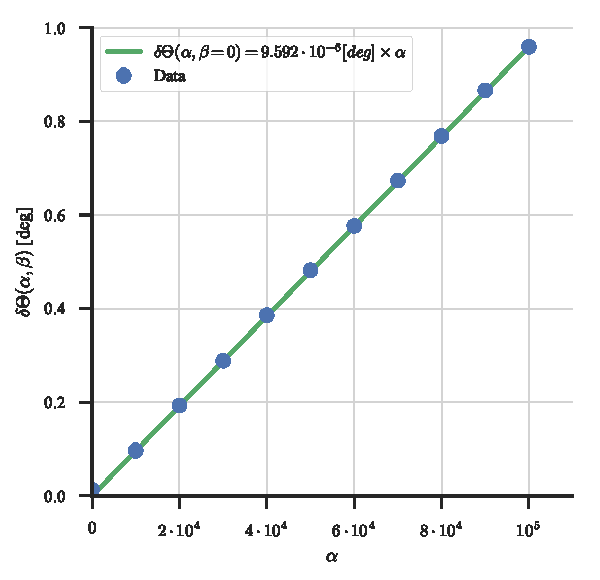
\includegraphics[width=\textwidth]{figs/alpha-angle.pdf}
		\caption{\label{fig:angle-alpha}}
	\end{subfigure}
	\begin{subfigure}[c]{0.49\textwidth}
		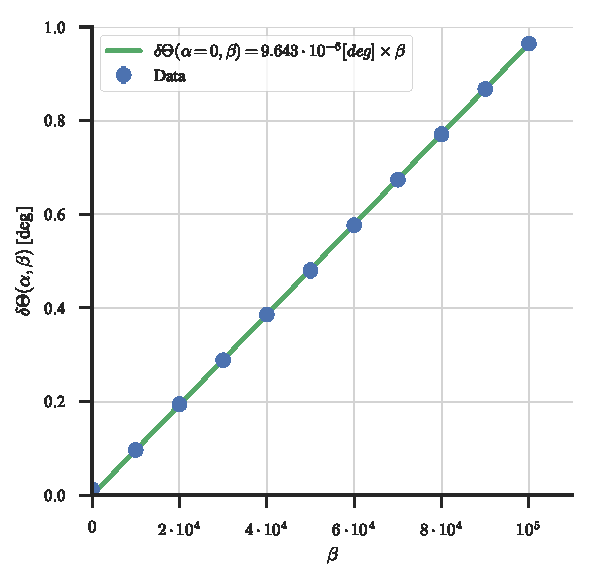
\includegraphics[width=\textwidth]{figs/beta-angle.pdf}
		\caption{\label{fig:beta-alpha}}
	\end{subfigure}
	\caption{\label{fig:AlphaAngle} Linear relation between $\alpha$ (a), $\beta$ (b) and the perihelion motion $\delta \Theta$ for $\Delta t=2v_M(0)/a_M(0)/200$ and the other parameter set to zero.}
\end{figure}

As an example we  extract the perihelion motion using the parameters provided by General Relativity, namely $\alpha = 0$ and $\beta = 3$.
Considering one result from the numeric simulation, e.g., $\delta\Theta(\alpha = 0, \beta=10^5) = 0.964^{\degree}$, the sought-after angle can be calculated by a linear interpolation as
\begin{equation}
	\delta\Theta (\alpha=0, \beta=3) = \frac{0.964^{\degree}}{10^5} \times 3 = 0.104''
	\, .
\end{equation}
Depending on the knowledge of the students, multiple points and also estimated numerical uncertainties could be used to extract this value by a linear regression.
Here, one has to find a proper range for the interpolation.
Small values for $\alpha$ and $\beta$ usually come with relatively larger numerical errors while for larger values one cannot guarantee that the additional terms are sufficiently small.
For this reason, we suggest to interpolate between zero and $\alpha_{\max}$, $\beta_{\max} \sim 10^5$.
This will be further explained in the next section.
Note that, when comparing the results of the simulation with the experimental result, one Earth year corresponds to $T_E/T_M \approx 365d/88d\approx 4.15$ Mercury years.
Therefore, the perihelion motion per 100 earth years is $0.104''\cdot 415\approx 43.2''$.
This is close to the experimental value of $\delta\Theta_{\mathrm{exp}} = 43.0''$.



%%%%%%%%%%%%%%%%%%%%%%%%%%%%%%%%%%%%%%%%%%%%%%%%%%%%%%%%%%%%%%%%%%%
\section{Tests of stability and error analysis}\label{sec:stability}
%%%%%%%%%%%%%%%%%%%%%%%%%%%%%%%%%%%%%%%%%%%%%%%%%%%%%%%%%%%%%%%%%%%
Measurements as well as numerical simulations in physics should always be accompanied by estimates of the corresponding uncertainties.
It is important for the students to recognize this fact and to understand that one cause of the uncertainties lies, e.g., in the finite time steps.
The students should therefore explore sources and sizes of inaccuracies arising in this simulation at least qualitatively.

There are many potential sources of uncertainties in a simulation and discussing all of them is be beyond the scope of this work.
Instead, we focus on the most accessible source, numerical errors due to finite time steps $\Delta t$.
Additional sources of errors include the omission of terms in Eqs.~(\ref{eq:vdef}) and~(\ref{eq:adef}) and the infinite mass approximation of the Sun (i.e.\ keeping the Sun's position fixed).

Consider figure~\ref{fcc3}, where the angle of the perihelion motion $\delta \Theta$ is shown for the first $10$ turns ($x$-axis) for different choices of $\Delta t$ (colors) and $\beta$ (columns). In all cases $\alpha=0$.
As expected, $\delta\Theta$ is approximately constant for sufficiently small time-steps $\Delta t$ and its value depends solely on $\beta$.
$\delta\Theta$ deviates from the expected value of zero for $\alpha = \beta = 0$.
Using the data points in figure~\ref{fig:AlphaAngle} and extrapolating to $\alpha=\beta=0$ without enforcing $\delta\Theta(0,0) = 0$ leads to a similar offset.
This offset is a numerical error and can be taken as an estimate for the error of the simulation.

\begin{figure}[htb]
	\centering
	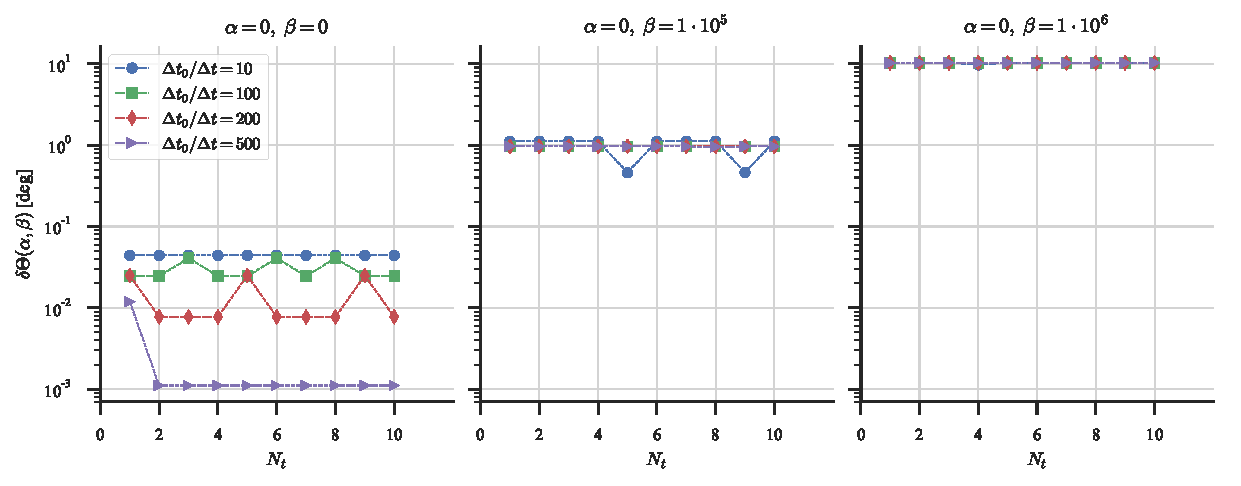
\includegraphics[width=.99\textwidth]{figs/angular-variaton.pdf}
	\caption{\label{fcc3}Motion of perihelion $\delta\Theta$ in degrees depending on the number of turns $N_t$ for different time steps $\Delta t$ (color) and different values for $\beta$ (columns).
	Here, $\Delta t_0 \equiv 2 v_M(0)/a_M(0)$.
	Offsets of $\delta \Theta(\alpha=0, \beta=0)$ from zero can be used as an estimated of the magnitude of the error. Oscillations in $\delta \Theta$ indicate too coarse time steps.
}
\end{figure}

Furthermore, one can observe that for large time-steps the values of the perihelion motion oscillate between discrete values at different turns.
This can be explained as follows: The sample code we present to find the perihelion vectors only finds the position closest to the Sun.
This is not the true perihelion but only an approximation to it. Sometimes the program finds a point before and sometimes after the perihelion which causes the observed oscillations.
The precision of this approximation rises as the time-step shrinks.
Hence, strong visible oscillations in $\delta\Theta$ indicate a too large time-step.

This problem can be pointed out to the students by asking them to vary the size of the time-steps and observe the effect on the trajectories.
This should also be done for a wide range of values to show both good and problematic regimes.
It is advantageous to set both $\alpha$ and $\beta$ to zero for this study, since in this case the trajectories should be closed and deviations from the correct case can be spotted easily.
Figure~\ref{fig:MercuryOrbit-a0-small-dt-large} shows the Mercury trajectory for $\Delta t=2 v_M(0) /a_M(0) \times 2$.
One can clearly see the failure of the simulation to reproduce the physical trajectory.
From examples like this it should be apparent that the time steps influence the accuracy of the simulation.
The simulation reproduces the actual trajectory only in the limit $\Delta t \rightarrow 0$. Thus, in any numerical simulation
one always has to identify a proper compromise between numerical accuracy and time spent for the simulation
(clearly for $\Delta t\to 0$ the computing time goes to infinity).

As a first estimate, one can approximate the numerical uncertainty of the the perihelion growth $\Delta \delta \Theta (\alpha, \beta)$ at non-zero $\alpha$ and $\beta$ by the offset of the growth at $\alpha = 0 = \beta$, the oscillation of the growth at $\alpha = 0 = \beta$ as well as the oscillation of the growth at the computed values for non-zero $\alpha$ and $\beta$
\begin{eqnarray}\label{eq:num-uncertainty}
	\Delta \delta \Theta (\alpha, \beta) &=& \sqrt{
		\delta \Theta_{mean}^2 (0, 0) + 
		\delta \Theta_{std}^2 (0, 0) + 
		\delta \Theta_{std}^2 (\alpha, \beta)
	} \, ,
	\\
	\delta \Theta_{mean} (\alpha, \beta)
	&=& 
	\frac{1}{N_{t}}
	\sum\limits_{n=1}^{N_{t}} \delta \Theta_{n} (\alpha, \beta) \, ,
	\\
	\delta \Theta_{std}^2 (\alpha, \beta)
	&=& 
	\frac{1}{N_{t}}
	\sum\limits_{n=1}^{N_{t}} \left[
		\delta \Theta_{mean} (\alpha, \beta) - \delta \Theta_{n} (\alpha, \beta)
	\right]^2 \, ,
\end{eqnarray}
where the standard deviations and mean values are obtained from the data sample of $N_t$ turns (orbits of mercury).
Thus, the extract numerical value is given by
\begin{equation}\label{eq:num-vals}
	\delta \Theta (\alpha, \beta) = \delta \Theta_{mean} (\alpha, \beta)  \pm \Delta \delta \Theta (\alpha, \beta)
	\, .
\end{equation}
Note that this has to be repeated for each different time step $\Delta t$.

The absolute value of the numerical error mostly depends on the tilmestep $\Delta t$ and is roughly independent on the values of $\alpha$ and $\beta$.
Therefore, it is more desirable to pick large values for $\alpha$ and $\beta$, because this increases the absolute value of the precision growth and thus decreases the relative numerical error.
However, there is a competing effect which places upper bounds on the values of $\alpha$ and $\beta$.
For instance, the prediction for the precision growth coming from General Relativity for zero $\alpha$ is given by
\begin{equation}\label{eq:gr-prediction}
	\delta \Theta_{GR} (\alpha=0, \beta) = 
	2 \pi \left[
	\frac{\beta}{4} \,\frac{r_S^2}{r_a^2}
	+\mathcal{O}\left(\beta^2\,\frac{r_S^4}{r_a^4}\right)
	\right]
	\, .
\end{equation}
Thus, once $\beta$ is sufficiently large, quadratic corrections in $\beta$ become relevant and it is not possible to extract the perihelion growth of Mercury by performing a linear interpolation.
We display these competing effects in Figure \ref{fcc4}.
The relative difference between numerically extracted values and the General Relativity prediction for $\delta \Theta$ are plotted against $\beta$ for zero $\alpha$.
While for smaller $\beta$, the relative numerical uncertainty grows, for larger $\beta \gtrsim 10^5$, the numerical values deviate from the linear prediction.
This is expected, because the non-linear corrections start to enter the percent regime
\begin{equation}
	\frac{\beta^2 \, r_S^4 / r_a^4}{\beta \, r_S^2 / r_a^2} \Bigg|_{\beta = 10^5}
	\sim
	1 \%
	\, .
\end{equation}
Identifying a parameter space for reliable and precise computations is a general challenge for numerical simulations.
\begin{figure}[htb]
	\centering
	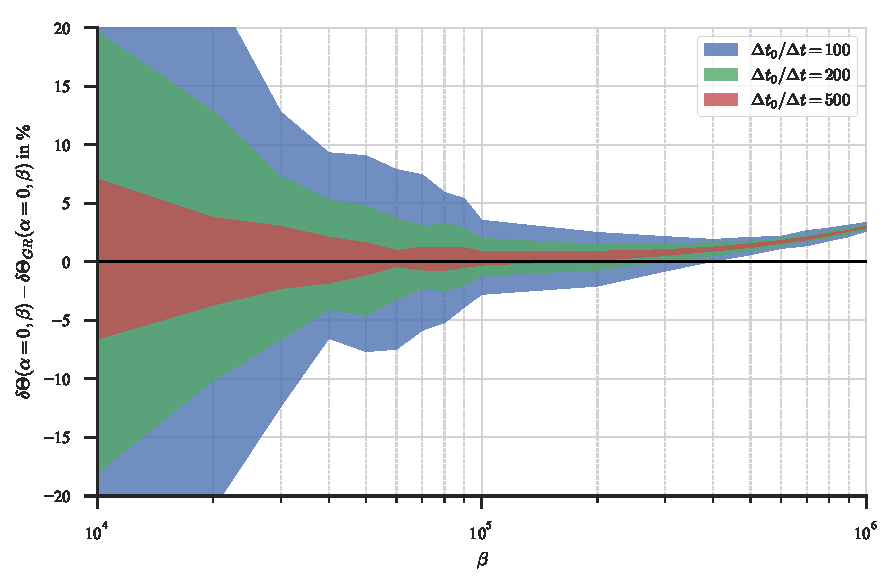
\includegraphics[width=.99\textwidth]{figs/computation-precision.pdf}
	\caption{\label{fcc4}Difference of numerically extracted perihelion angle growth relative to value computed from General Relativity [Equation (\ref{eq:gr-prediction})] for different time steps.  The error bands are the envelope for computed data points where the size of the error is determined according to Equation (\ref{eq:num-vals}).
}
\end{figure}


%%%%%%%%%%%%%%%%%%%%%%%%%%%%%%%%%%%%%%%%%%%%%%%%%%%%%%%%%%%%%%%%%%%
\section{Dimensional analysis}\label{sec:analysis}
%%%%%%%%%%%%%%%%%%%%%%%%%%%%%%%%%%%%%%%%%%%%%%%%%%%%%%%%%%%%%%%%%%%

Dimensional analysis is not only a tool that allows one to cross check if the results of some simulation is of the right order of magnitude, it is also very helpful to identify unusual dynamics in some system.
Especially the latter aspect should become clear from the discussion in this section.

The idea of dimensional analysis is that in a system that can be controlled by expanding the relevant quantities (like the force) in some small parameter(s), the coefficients in the expansion should turn out to be of order one (that means anything between about 0.1 and 10 is fine --- but 0.01 or 100 is irritating); parameters in line with this are called "natural".
Applied to the problem at hand given by Eq.~(\ref{eq:newton}) this statement implies that from naturalness one would expect the parameters $\alpha$ and $\beta$ of order one when $r$ is about the average distance Mercury-Sun, namely $\bar r=6\times 10^7\,\mathrm{km}$.
From this one estimates for the expected angular shift per orbit for $\alpha=1$ and $\beta=0$
\begin{equation}
\delta \Theta \simeq 2\pi\left(\frac{r_S}{\bar r}\right) = (\pi \times 10^{-7}) \ \mbox{rad} = (2\cdot 10^{-5})^o = (7\cdot 10^{-2}) ^{''} \ ,
\end{equation}
or for $\alpha=0$ and $\beta=1$
\begin{equation}
\delta \Theta \simeq 2\pi\left(\frac{a^2}{\bar r^2}\right) = (\pi \times 5 \cdot 10^{-8}) \ \mbox{rad} = (1 \cdot 10^{-5})^o = (4\cdot 10^{-2}) ^{''} \ ,
\end{equation}
which leads to a shift of about $30^{''}$ and $15^{''}$, respectively, in 100 earth years. These are to be compared to the empirical value of $43^{''}$.
Thus the amount of perihelion motion of Mercury is indeed in line with expectations, \textit{if} --- and this is an important "if" --- the Newtonian dynamics is simply the leading term of some more general underlying theory.
In particular, no new scales enter in the correction terms in addition to $r_S$ and $r_a^2$.

Thanks to Einstein we indeed know that the conclusion formulated above is correct; the more general underlying theory is General Relativity and Einstein was able to explain the perihelion motion of Mercury from his equations quantitatively.
On the other hand, had we found the need for a dramatic deviation of the parameters from unity one would have concluded that there is probably some other dynamics that drives this difference.

Indeed, nowadays there are  several of those hierarchy problems in modern physics: e.g., the so called QCD $\Theta$ term, expected to be of natural size, is at present known to be at most $10^{-10}$.
This smallness, called the strong CP problem, is so irritating that physicists like S. Weinberg even proposed that there must exist an additional particle, the axion.
Its interactions would even push $\Theta$ to zero.
At present various intense experimental searches for this axion are going on at various labs.



%%%%%%%%%%%%%%%%%%%%%%%%%%%%%%%%%%%%%%%%%%%%%%%%%%%%%%%%%%%%%%%%%%%
\section{Possible extensions}\label{sec:extensions}
%%%%%%%%%%%%%%%%%%%%%%%%%%%%%%%%%%%%%%%%%%%%%%%%%%%%%%%%%%%%%%%%%%%

\begin{itemize}

\item \textbf{Explore Problem autonomously}

In chapter~\ref{sec:Numerical Implementation} we suggested to present the material by using a template as well as a step by step instruction to guide the students through the problem solution.
These instructions can be cut down or left out depending on available time and numerical/computational versatility of the students.
This could be achieved by the following changes or additions to the concept presented in chapter \ref{sec:Numerical Implementation}.

\begin{itemize}
\item \textbf{Build code from scratch}

Instead of providing the template to the students, they could build the program from scratch.
Of course, this requires some basic knowledge in \vpython{}, which they could acquire for example by working through "a ball in a box" (see~\cite{VPythonIntro}) or similar tutorials.
Also, they could independently research the parameters relevant for the system.
\item \textbf{Why can we work in one plane?}

In the code the third coordinate of all vectors is set to zero and never used.
On the first glance, this might seem like a simplification.
This choice is however possible without loss of generality because we are dealing with a central potential.
The students could work out the reason behind this choice on their own.
\item \textbf{What is the impact of the different parameters?}

Especially if the parameters are not specified beforehand, the students might have to experiment a bit, before getting the correct trajectories.
But even if they are given, it might be beneficial to encourage the students to play with a few parameters, like the masses or the starting velocities, and observe their impact on the trajectories.
This way the students get a better feeling for the physics involved.
\end{itemize}

\item \textbf{Optimizing performance}

Simulations always involve a balance between time needed for the calculations and the demanded accuracy for the results.
Even though this is a rather simple example, it contains some opportunities to make these concepts accessible to the students.

\begin{itemize}
\item \textbf{Measure calculation time}

In practice there is a limit to decreasing the time steps, because the time needed for the calculation grows simultaneously.
The following snippet shows how the run time of function \texttt{main} can be measured:
\begin{lstlisting}
import time
start_time = time.time()
main()
print("--- {} seconds ---".format(time.time() - start_time))
\end{lstlisting}
By varying $\Delta t$ they can validate, that there is indeed approximately an anti-proportional dependence.
(Note: This only works if the time in the loop is increased by $\Delta t$, so $t=t+\Delta t$.)
\item \textbf{Verlet integration}

Obviously, an improvement in accuracy can be achieved by using a better algorithm without changing $\Delta t$.
The simplest way to demonstrate this might be given by the implementation of the Verlet (see e.g.~\cite{Hairer03geometricnumerical} and references therein) integration instead of using the simple Euler method.
\end{itemize}

\item \textbf{Extended Problems}

\begin{itemize}
\item \textbf{Non-stationary Sun}

It might be interesting to abandon the simplification of a stationary Sun, as it nicely illustrates Newton's third law.
Here it might also be advisable to reduce the mass of the sun to have a more visible result.

\item \textbf{Three-body problem}

Ambitious students could even include further planets and see how the different planets interact.
This is especially interesting, when discussing the perihelion motion of Mercury, as it is mainly due to the influence of the other planets.
Only a smaller part is due to General Relativity.

\end{itemize}

\end{itemize}

\todo[inline]{Summary}



%%%%%%%%%%%%%%%%%%%%%%%%%%%%%%%%%%%%%%%%%%%%%%%%%%%%%%%%%%%%%%%%%%%
\section*{Acknowledgments}

This work is supported in part by NSFC and DFG through funds provided to the
Sino--German CRC110 ``Symmetries and the Emergence of Structure in QCD''.


%%%%%%%%%%%%%%%%%%%%%%%%%%%%%%%%%%%%%%%%%%%%%%%%%%%%%%%%%%%%%%%%%%%
%\section*{References}
%%%%%%%%%%%%%%%%%%%%%%%%%%%%%%%%%%%%%%%%%%%%%%%%%%%%%%%%%%%%%%%%%%%

\appendix
%%%%%%%%%%%%%%%%%%%%%%%%%%%%%%%%%%%%%%%%%%%%%%%%%%%%%%%%%%%%%%%%%%%
\section*{References}
\bibliographystyle{unsrt}%{alphadin}
\bibliography{References}


%%%%%%%%%%%%%%%%%%%%%%%%%%%%%%%%%%%%%%%%%%%%%%%%%%%%%%%%%%%%%%%%%%%
\clearpage
\section{The complete code}\label{sec:code}
%%%%%%%%%%%%%%%%%%%%%%%%%%%%%%%%%%%%%%%%%%%%%%%%%%%%%%%%%%%%%%%%%%%
Below we provide the complete code as developed above.
\lstinputlisting[language=Python,basicstyle=\linespread{1}\scriptsize\ttfamily]{mercury_orbit_base.py}
Further examples and template files can be found online \cite{scripts}.

\end{document}
